\documentclass[a4paper,titlepage,12pt]{article}
\usepackage[utf8]{inputenc}
\usepackage[T1]{fontenc}
\usepackage{lmodern}
\usepackage[magyar]{babel}
\usepackage{graphicx}
\usepackage{float}
\usepackage{amsmath}
\begin{document}

	\begin{centering}
		\scshape\LARGE Folytonos közegek mechanikája (emelt szint) \par
		\vspace{1cm}
		
		\large 7. tétel: Felületi feszültség, görbületi nyomás, kapilláris emelkedés
	\end{centering}
		
\part{Felületi feszültség}

Megfigyelés: Fém kereten szappanhártya feszül, a keresztben lévő l hosszúságú drót elmozdulhatna, ezért F erőt kell alkalmazni az egyensúlyhoz. Ennek az erőnek a nagysága függ az anyagi minőségtől, és a keretben lévő szál hosszától. $$ F=2\alpha\cdot l $$

\noindent
Ebben a képletben $\alpha$-t felületi feszéltségnek nevezzük, és a  mértékegysége: $ \frac{N}{m}$ . 
\vspace{0.5 cm}

\noindent
Most a keretet mozdítsuk el egy $\Delta x$ távolsággal. A mozgatáshoz szükséges erő ebben az esetben nem változik. Így a végzett munkát a következő alakban írhatjuk le: $$\Delta W=F \Delta x=\alpha 2l \Delta x = \alpha \Delta A $$ 

\begin{figure}[H]
	\begin{center}
		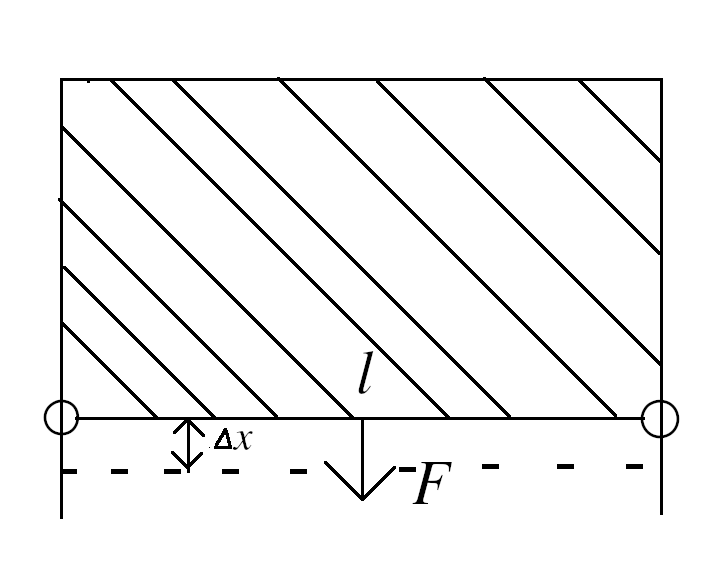
\includegraphics[width=0.4\textwidth]{tetel7.png}
		\caption{A fémkeret, benne a hártyával. F erővel $\Delta x $ távolsággal kihúzzuk.}
	\end{center}
\end{figure}

\noindent
A felületi feszültségre ebből a képletből adódik az alábbi alak: $$\alpha=\frac{dW}{dA}$$

\noindent
A felületi feszültség minden határfelületen fellép. Energetikai szempontból a minimális határfelületű alakzatok a legkedvezőbbek, ezért a hártya mindig abba az alakba igyekszik beállni. Ezt megfigyelhettük az előadáson, amikor szappanhártyákat vizsgáltunk különböző alakú testeknél. 

\part*{Görbületi nyomás}

Egy üveglapra vízcseppet ejtünk. Legyen $\alpha$ az egységnyi hosszra ható erő. $A$ pont egyensúlyban van. Vízszintes irányban az egyensúly:
\[\alpha_{\text{vü}}+\alpha_{\text{vl}}\cdot\cos{\varphi}-\alpha_{\text{ül}}\]

\noindent
Az illeszkedési egyenlet pedig: \[\cos{\varphi}=\frac{\alpha_{\text{ül}}-\alpha_{\text{vü}}}{\alpha_{\text{vl}}}\]

\noindent
Hogyha ennek az egyenletnek az eredménye nagyobb mint 1, akkor nem lehet egyensúlyban a pont, tehát a vízcsepp elfolyik.

\begin{figure}[H]
	\begin{center}
		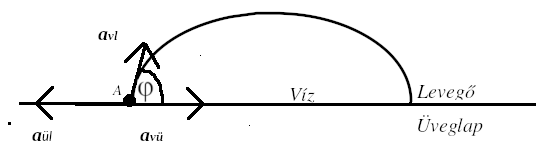
\includegraphics[width=0.7\textwidth]{tetel72.png}
		\caption{Az üveglapon lévő vízcsepp, rajta A egyensúlyban lévő ponttal és a rá ható erőkkel}
	\end{center}
\end{figure}

\noindent
Mivel a felületi feszültségek függnek a hőmérséklettől, előfordulhat, hogy bizonyos tartományokon van megoldás, más tartományokon nincs. Hogyha ezt az egyenletet felírjuk a tinta, levegő és papír esetére, akkor magyarázatot kapunk a toll működésére.

\part*{Görbített határfelület}

\begin{figure}[H]
	\begin{center}
		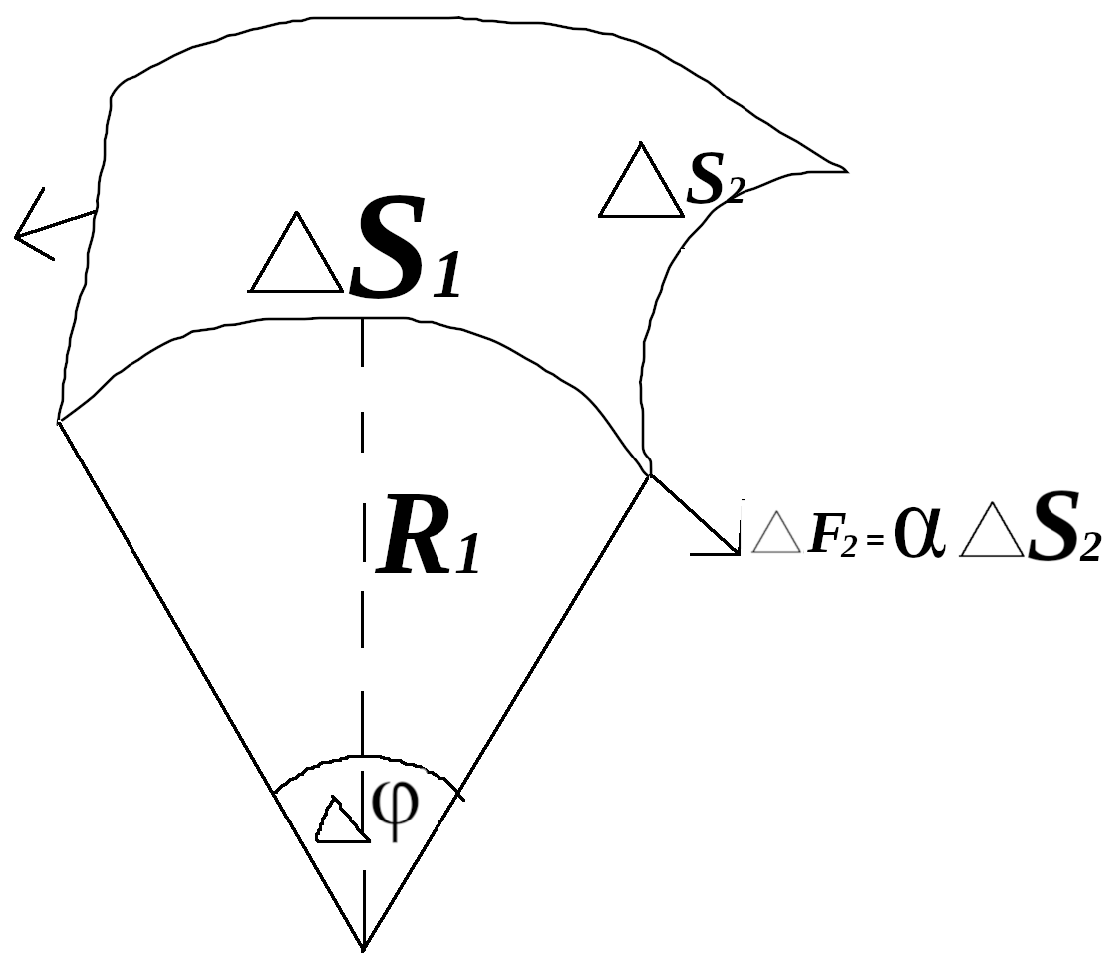
\includegraphics[width=0.4\textwidth]{tetel73.png}
		\caption{Egy kifeszített $\alpha$ felületi feszültségű görbe hártya. }
	\end{center}
\end{figure}

\noindent
A felület szélein fellépő $\Delta F_{2}$ erők függőleges komponense: $$ \Delta F_{2_{f}} =2\alpha\Delta S_{2}\cdot\sin{\frac{\Delta\varphi}{2}}=\alpha\Delta S_{2}\cdot\Delta\varphi=\alpha\Delta S_{2}\Delta S_{1} \frac{1}{R_2} $$

\noindent
Mivel a másik szélnél is lép fel erő, így a teljes függőleges erőre az alábbi képlet adódik: $$ \Delta F_{f}=\alpha(\frac{1}{R_{1}}+\frac{1}{R_{2}})\Delta S_{1}\Delta S_{2} $$

\noindent
A $\Delta F_{f}$-et kompenzálhatja a nyomáskülönbség. $$ \Delta F_{f}=p\Delta A=p\Delta S_{1}\Delta S_{2}$$

\noindent
A gömbfelületi nyomásra így a következő egyenletet kapjuk: $$p_{g}=\alpha(\frac{1}{R_{1}}+\frac{1}{R_{2}}) $$

\noindent
Ebből is látszik, hogy kisebb sugarú gömb esetén a gömbfelületi nyomás nagyobb. Szilárd anyagok esetén a nyomás helyett a feszültségtenzor használata a célszerű. A feszültségtenzor a határon ugrik.

\part*{Kapilláris emelkedés }

\begin{figure}[H]
	\begin{center}
		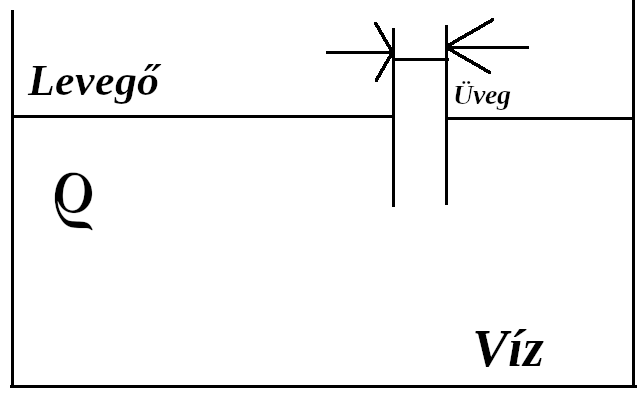
\includegraphics[width=0.3\textwidth]{tetel74.png}
		\caption{A vízbe merített kapilláris csőben a víz magasabban áll, mint az edényben.}
	\end{center}
\end{figure}

\noindent
Az emelkedés energetikai leírása: $$ W(h)=r^{2}h\varrho g \frac{h}{2}+2r\pi h\alpha_{uv}-2r\pi h\alpha_{ul}$$

\noindent
Ahol $\frac{h}{2}$ a tömegközéppont emelkedése.

\noindent
Ez akkor lesz egyensúlyban, ha a $W(h)$ függvénynek minimuma van, azaz: $$\frac{dW}{dh}=0=r^2\pi\varrho gh+(\alpha_{uv}-\alpha_{ul})2r\pi=0 $$ 

\noindent
Amit egyszerűsítve és átrendezve az alábi képletet kapjuk: $$h=\frac{2(\alpha_{ul}-\alpha_{uv})}{\varrho gr}=-\frac{\alpha_{vl}\cos{\varphi}}{\varrho gr}$$

\noindent
Ahol $\varphi$ az illeszkedési szög.

\noindent
Valójában a kialakuló folyadék felülete nem vízszintes, de ez a $\Delta h$ elhanyagolható a h-hoz képest.

\noindent
A $h$ lehet negatív is, például a higanynál.

\noindent
A képletben is látszik az, amit már tapasztalatból megfigyelhettünk, azaz hogy az emelkedés vastag csőben elhanyagolható.


\end{document}